\documentclass{article}
\usepackage{amsmath}
\usepackage[backend=biber, style=apa,]{biblatex}
\usepackage{booktabs}  % Required for \toprule, \midrule, \bottomrule, and \cmidrule
\usepackage{caption}
\usepackage{csquotes}
\usepackage[left=2.54cm,right=2.54cm,top=2.54cm,bottom=2.54cm]{geometry}
% \usepackage[draft]{graphicx} % Draft mode
\usepackage{graphicx}
\usepackage{setspace}
\usepackage{subcaption}
\usepackage{tikz}
\usetikzlibrary{shapes.geometric, arrows.meta, positioning, calc}

\usepackage{xeCJK}


\setCJKmainfont{MS Mincho} % Or any Japanese font on your PC

\addbibresource{bibliography.bib} %Imports bibliography file

\begin{document}
\onehalfspacing{}

\title{Bachelor Thesis}
\author{Mikael Wijaya}
\date{\today}

\maketitle
\newpage

\tableofcontents
\newpage

% Use \include or \input to call your sections
\section{Introduction}

\subsection{Background}
Air pollution in urban areas represents an ongoing global challenge that negatively impacts individual health, ecosystem integrity, and places increasing pressure on medical systems and economies worldwide. Urban air pollution comprises multiple components, including carbon dioxide (CO$_2$), carbon monoxide (CO), and particulate matter with an aerodynamic diameter of less than 2.5 $\mu$m (PM$_{2.5}$). 

The health implications are severe; recent data from the \textcite{WHO2024Ambient} indicates that ambient air pollution contributes to approximately 4.2 million premature deaths globally each year. While mortality is largely attributed to increased private vehicle demand and population growth, a significant contributing factor is the lack of consideration for pollutant dispersion during rapid urban development \parencite{Li2021Review}. As noted by \textcite{Li2021Review}, "hasty and irrational construction strategies" often lead to poor ventilation, trapping pollutants in high concentrations near the ground level.

Understanding and mitigating these concentrations requires a dual-level approach. First, it involves the utilization of mechanical factors, which include forced convection by wind, natural convection by solar radiation, and traffic-induced turbulence. Second, it requires the strategic design of urban morphology. This focus on the "sound design of the urban landscape" emphasizes building geometries, urban density, and enclosure degrees to improve the city's natural capacity to flush out pollutants \parencite{Li2021Review}.

The morphology and organization of urban areas directly influence urban traffic patterns and pollutant flow dynamics. Therefore, understanding the relationship between urban morphology, pollutant transport, and air quality is critical for developing effective mitigation strategies that move beyond qualitative observations toward quantitative air quality improvements.


\newpage
\subsection{Objective}


\newpage

\section{Theory}

\subsection{Lattice Boltzmann Method}

To simulate urban air pollutant transport, this study employs the Lattice Boltzmann Method (LBM), a mesoscopic computational fluid dynamics (CFD) technique. Unlike traditional solvers that directly discretize the macroscopic Navier-Stokes equations, LBM models fluid flow by simulating the collective behavior of a distribution of particles on a discrete grid, or "lattice" \parencite{Kruger2017LBM}.The movement of these particles is governed by the Lattice Boltzmann Equation (LBE), which describes the evolution of the discrete-velocity distribution function $f_i$:

\begin{equation}
    f_{i}(\mathbf{x} + \mathbf{c}_{i}\Delta t, t + \Delta t) - f_{i}(\mathbf{x}, t) = \Omega_i(f) + S_i    
\end{equation}

Where $f_i$ is the distribution function representing the density of particles moving with velocity components $\mathbf{c}_i$ in the $i$-th direction. The term $\Omega_i$ represents the collision operator, which models the internal redistribution of particle momentum, while $S_i$ is the source term. The inclusion of $S_i$ is critical for this research as it allows for the integration of external body forces and the modeling of mass sources, such as vehicle emissions.The simulation proceeds through a sequence of two primary operations: streaming and collision. During the streaming step, particles move from their current node $\mathbf{x}$ to adjacent points based on their respective velocities. Following this, the collision step redistributes the particle velocities at each node based on local interactions, effectively mimicking fluid viscosity and relaxation toward equilibrium. As noted by \textcite{Kruger2017LBM}, LBM offers several distinct advantages for simulating complex urban environments. First, the underlying Boltzmann equation is essentially a hyperbolic advection equation where the source terms depend only on local values of $f$. Because these operations rely strictly on information from a node and its immediate neighbors, the algorithm is inherently local. This locality facilitates high-performance parallelization, which is essential for large-scale urban simulations. Furthermore, the grid-based nature of LBM allows for the efficient handling of complex building geometries and irregular urban morphologies without the need for the intensive re-meshing often required by finite-element methods.

\subsubsection{Lattice Configuration and Accuracy}
The choice of the D3Q27 lattice model is fundamental to the accuracy of the turbulence modeling in this research \parencite{Yokouchi2020Simulation}. While the simpler D3Q19 model is often used to reduce computational costs, it lacks the rotational invariance required to capture complex secondary flows accurately. As demonstrated by \textcite{Suga2015D3Q27}, the D3Q27 lattice provides a superior representation of turbulent structures. Their comparative analysis of turbulent pipe flow showed that the D3Q27 model produces significantly more realistic flow fields than the D3Q19 model, which tends to struggle with resolving fine-scale turbulent fluctuations in three-dimensional space. By utilizing 27 discrete velocities, the model can more effectively resolve the secondary circulations and high-frequency fluctuations necessary for an in-depth understanding of the pollutant dispersion mechanism in urban areas.The internal redistribution of particle momentum is governed by the Bhatnagar-Gross-Krook (BGK) collision operator. This operator assumes that the particle populations relax toward a local equilibrium state, $f_i^{eq}$, at a rate controlled by a single relaxation time $\tau$ \parencite{Kruger2017LBM}:

\begin{equation}
    \Omega_i(f) = -\frac{f_i - f_i^{eq}}{\tau}\Delta t    
\end{equation}

The equilibrium distribution $f_i^{eq}$ is formulated as a second-order expansion of the Maxwell-Boltzmann distribution in terms of the macroscopic density $\rho$ and velocity \textbf{u}:
\begin{equation}
    f_i^{eq}(\mathbf{x},t) = w_i \rho \left( 1 + \frac{\mathbf{u} \cdot \mathbf{c}_i}{c_s^2} + \frac{(\mathbf{u} \cdot \mathbf{c}_i)^2}{2c_s^4} - \frac{\mathbf{u} \cdot \mathbf{u}}{2c_s^2} \right)    
\end{equation}

Here, $c_s$ represents the isothermal speed of sound, defined as $c_s^2 = \frac{1}{3}\frac{\Delta x^2}{\Delta t^2}$. This formulation ensures the local conservation of mass and momentum while establishing the relationship between pressure and density as $p = c_s^2 \rho$.

\subsubsection{Large Eddy Simulation and Turbulence Modeling}
To capture the transient, multi-scale nature of urban wind flows, this research utilizes a Large Eddy Simulation (LES) approach. The unresolved subgrid-scale (SGS) motions are accounted for using the Coherent-structure Smagorinsky Model (CSM). In a standard Smagorinsky framework, the turbulent viscosity $\nu_t$ is determined by the strain-rate tensor $|S|$ and a filter width $\Delta$:

\begin{equation}
    \nu_t = (C_S\Delta)^2|S|    
\end{equation}

Within the LBM framework, the total viscosity $\nu$ (the sum of molecular and turbulent viscosity) is directly linked to the relaxation time:

\begin{equation}
    \nu = c_s^2 \left(\tau - \frac{\Delta t}{2} \right)    
\end{equation}

While a standard Smagorinsky constant $C_S$ typically ranges between 0.1 and 0.2 \parencite{Blazek2015CFD}, the CSM used here employs a dynamic parameter based on the second invariant of the velocity gradient tensor. This approach allows the model to automatically account for wall-damping effects, ensuring more accurate flow predictions near building surfaces without requiring manual damping functions \parencite{Phuc2018CSM}.

\subsubsection{Implementation of Lagrangian Stochastic Model}
To simulate the transport and dispersion of particulate matter within the urban environment, this study utilizes a Lagrangian Stochastic Model (LSM). Unlike Eulerian methods that treat pollutants as a continuous concentration field, the LSM tracks the trajectories of thousands of discrete "passive" particles within the turbulent flow field generated by the LBM. This approach is particularly effective for modeling dispersion in the inhomogeneous and non-Gaussian turbulence characteristic of the urban planetary boundary layer (PBL). By simulating a statistically significant ensemble of particle paths, the ensemble-mean concentration can be derived, which is directly proportional to the particle number density or the probability density function (PDF) of particle positions \parencite{Weil2024LSM}.The trajectory of each particle is determined by integrating its position $x_p$ over time. For a particle starting at an initial position $x_0$, the position at the next time step $t + \Delta t$ is calculated as:

\begin{equation}
    x_p(x_0, t + \Delta t) = x_p(x_0, t) + u_p(x_0, t)\Delta t    
\end{equation}

where $u_p$ represents the instantaneous Lagrangian particle velocity. This velocity is composed of two primary components: $$u_p = u_r + u_s$$ 
In this formulation, $u_r$ is the resolved grid-scale (GS) velocity obtained directly from the LBM-LES results, representing the large-scale atmospheric motions. The term $u_s$ represents the subgrid-scale (SGS) velocity fluctuations, which account for the smaller, unresolved turbulent motions.The resolved velocity $u_r$ at the particle's location is determined by interpolating the LBM grid results using the weighting factors $w_i$ of the neighboring nodes: $$u_r = \sum_{i=0}^7(w_i U_i)$$

To account for the unresolved fluctuations, the SGS velocity $u_s$ is modeled as a stochastic process. Following the framework established by \textcite{Weil2024LSM} and \textcite{Thomson1987Stochastic}, the evolution of the SGS velocity $du_s$ is described by a stochastic differential equation: 

\begin{equation}
    du_s = -\frac{3f_sC_0\epsilon}{4}dt + \frac{1}{2}\left( \frac{1}{e_s}\frac{de_s}{dt}u_s + \frac{2}{3}\nabla e_s \right)dt + (f_sC_0\epsilon)^{1/2}d\xi
\end{equation}

where $e_s$ is the local SGS turbulent kinetic energy (TKE) and $f_s$ represents the mean contribution of the SGS TKE to the total TKE. The term $\epsilon$ denotes the total dissipation rate, while $C_0$ is a universal constant (set to 4.0 in this study). The stochastic component $(f_sC_0\epsilon)^{1/2}d\xi$ incorporates Gaussian white noise via the displacement vector $d\xi$, allowing the model to represent the random nature of sub-lattice turbulent dispersion.

\subsubsection{Advanced Wall Boundary Conditions}
In LBM, the standard Bounce-Back (BB) scheme assumes that fluid particles hitting a solid boundary reverse their momentum, effectively enforcing a no-slip condition ($\mathbf{u}=0$) at the wall. While numerically stable and simple to implement, the BB scheme requires the first grid point to reside within the viscous sublayer to accurately capture wall shear stress. In urban-scale simulations, the grid resolution is typically much larger than the thickness of this sublayer, causing the BB scheme to underpredict shear drag.To resolve this, a Wall Function Boundary (WFB) is implemented, following the approach evaluated by \textcite{Han2021WFB}. The WFB utilizes Spalding's Law to model the non-linear velocity profile in the logarithmic layer, allowing the simulation to approximate near-wall velocity without fully resolving the thin viscous region. This modification is applied during the collision step by introducing a momentum loss term based on the wall shear stress $\tau_w$:

\begin{equation}
    f_a^* = f_a \pm \frac{\Delta t}{2\Delta y}\tau_{w,j}
\end{equation}

where $\tau_{w,j}$ is the shear stress in the $j$-direction ($x$ or $z$). The wall shear stress is determined by solving Spalding's implicit equation:

\begin{equation}
    y^+ = u^+ + e^{-\kappa B} \left[ e^{\kappa u^+} - 1 - (\kappa u^+) - \frac{(\kappa u^+)^2}{2} - \frac{(\kappa u^+)^3}{6} \right]
\end{equation}

Here, $y^+$ is the dimensionless distance from the wall, and $u^+$ is the dimensionless velocity. By calculating the friction velocity $u_{\tau} = \sqrt{\tau_w / \rho}$ from this relationship, the model applies a "reverse resistance" that decelerates particles near building surfaces. As demonstrated by \textcite{Han2021WFB}, this WFB approach significantly improves the accuracy of shear drag predictions in high-Reynolds-number urban flows where coarse grids are a necessity.

\subsubsection{Subgrid-Scale Turbulent Kinetic Energy (SGS TKE)}
The calculation of the SGS TKE ($e_s$) is vital for the Lagrangian Stochastic Model, as it dictates the magnitude of the stochastic velocity fluctuations. While traditional LES often parameterizes $e_s$ via the eddy viscosity and a mixing length ($v_t = c_k l e_s^{1/2}$), this study utilizes a filtering approach as implemented by \textcite{Suga2015D3Q27} and \textcite{Yokouchi2020Simulation}. The SGS TKE ($k_{sgs}$) is derived from the difference between the instantaneous grid-scale velocity and a filtered velocity field:

\begin{equation}
    k_{sgs} = C_{kes} \sum_{i=1}^3 (\langle \hat{U}_i \rangle - \langle U_i \rangle)^2    
\end{equation}


The filtered velocity $\langle \hat{U}_i \rangle$ is calculated using a weighted average of the central node (50\% weight) and its six immediate neighbors (1/12 weight each):

\begin{equation}
    \langle \hat{U}_i \rangle = \frac{1}{2}\langle U_i \rangle + \frac{\langle U_i^E \rangle + \langle U_i^W \rangle + \langle U_i^N \rangle + \langle U_i^S \rangle + \langle U_i^T \rangle + \langle U_i^B \rangle}{12}    
\end{equation}

This local filtering operation is highly compatible with the LBM's neighbor-only communication pattern, maintaining the algorithm's high parallel efficiency while providing a robust estimate of local turbulence intensity.

\subsubsection{Stochastic Integration and Stability}
The stochastic component of the LSM involves the integration of Gaussian white noise, $\xi(t)$, which is formally defined as the time derivative of a Wiener process $W(t)$:

\begin{equation}
    W_i(t) = \int_0^t \xi(s) ds    
\end{equation}

In accordance with Brownian motion theory, the variance of this process increases linearly with time. Given that the SGS velocity $u_s$ is modeled as a random walk, the stochastic term $(f_s C_0 \epsilon)^{1/2} d\xi$ can occasionally produce unrealistically high instantaneous velocities. This is particularly prevalent near building walls where $e_s$ is high and the gradient terms in the LSM equation are steep. To prevent numerical instability and maintain physical consistency, a velocity limitation is enforced, ensuring that the total Lagrangian particle velocity $u_p$ remains within physically plausible bounds relative to the local mean flow \cite{Yokouchi2020Simulation}.

\subsubsection{Model Selection and Validation via Flat Plate Analysis}

Before applying the model to complex urban morphologies, \textcite{Yokouchi2020Simulation} conducted a validation study using particle dispersion over a flat plate to identify the most accurate combination of numerical schemes. The evaluation compared three primary configurations: (1) a baseline model using a simple Bounce-Back (BB) boundary and the standard subgrid-scale (SGS) model; (2) a model incorporating the Wall Function (WF) and Suga's refined SGS TKE calculation; and (3) an integrated model combining the WF-Suga framework with the Lagrangian Stochastic Model (LSM) and a velocity limitation.The accuracy of these models was evaluated based on their ability to replicate the theoretical logarithmic profile of particle concentration in a neutral boundary layer:

\begin{equation}
    \frac{C_0 - C}{C^*} = \frac{1}{\kappa} \ln \frac{z}{z_0}    
\end{equation}

where $C_0$ represents the particle density at ground level, $C^*$ is the friction density, $\kappa$ is the von Kármán constant, and $z_0$ is the roughness length.The results demonstrated that the WF-Suga-LSM model provided the highest correlation with the logarithmic profile. In contrast, models without the LSM or the specialized SGS TKE tended to deviate from the expected distribution, particularly in the near-wall region. Furthermore, the necessity of the speed limitation—defined as $|u_s| < k_{sgs}^{1/2}$—was confirmed through an analysis of the particle velocity variance. Without this limitation, the stochastic term in the LSM produced unrealistically high velocity fluctuations near the boundary. Implementing the speed limit successfully reduced this variance, ensuring a stable and physically consistent velocity distribution across the vertical profile.By adopting this validated WF-Suga-LSM framework with speed limitations, this research ensures that the fundamental transport mechanisms are correctly modeled before introducing the complexities of the AIJ Case H urban block.

\newpage
\section{Methodology}
\subsection{Lattice Boltzmann Method}

To simulate urban air pollutant transport, this study employs the Lattice Boltzmann Method (LBM), a mesoscopic computational fluid dynamics (CFD) technique. Unlike traditional solvers that directly discretize the macroscopic Navier-Stokes equations, LBM models fluid flow by simulating the collective behavior of a distribution of particles on a discrete grid, or "lattice" \parencite{Kruger2017LBM}.The movement of these particles is governed by the Lattice Boltzmann Equation (LBE), which describes the evolution of the discrete-velocity distribution function $f_i$:

\begin{equation}
    f_{i}(\mathbf{x} + \mathbf{c}_{i}\Delta t, t + \Delta t) - f_{i}(\mathbf{x}, t) = \Omega_i(f) + S_i    
\end{equation}
Where $f_i$ is the distribution function representing the density of particles moving with velocity components $\mathbf{c}_i$ in the $i$-th direction. The term $\Omega_i$ represents the collision operator, which models the internal redistribution of particle momentum, while $S_i$ is the source term. The inclusion of $S_i$ is critical for this research as it allows for the integration of external body forces and the modeling of mass sources, such as vehicle emissions.The simulation proceeds through a sequence of two primary operations: streaming and collision. During the streaming step, particles move from their current node $\mathbf{x}$ to adjacent points based on their respective velocities. Following this, the collision step redistributes the particle velocities at each node based on local interactions, effectively mimicking fluid viscosity and relaxation toward equilibrium. As noted by \textcite{Kruger2017LBM}, LBM offers several distinct advantages for simulating complex urban environments. First, the underlying Boltzmann equation is essentially a hyperbolic advection equation where the source terms depend only on local values of $f$. Because these operations rely strictly on information from a node and its immediate neighbors, the algorithm is inherently local. This locality facilitates high-performance parallelization, which is essential for large-scale urban simulations. Furthermore, the grid-based nature of LBM allows for the efficient handling of complex building geometries and irregular urban morphologies without the need for the intensive re-meshing often required by finite-element methods.

\subsubsection{Lattice Configuration and Accuracy}
The choice of the D3Q27 lattice model is fundamental to the accuracy of the turbulence modeling in this research \parencite{Yokouchi2020Simulation}. While the simpler D3Q19 model is often used to reduce computational costs, it lacks the rotational invariance required to capture complex secondary flows accurately. As demonstrated by \textcite{Suga2015D3Q27}, the D3Q27 lattice provides a superior representation of turbulent structures. Their comparative analysis of turbulent pipe flow showed that the D3Q27 model produces significantly more realistic flow fields than the D3Q19 model, which tends to struggle with resolving fine-scale turbulent fluctuations in three-dimensional space. By utilizing 27 discrete velocities, the model can more effectively resolve the secondary circulations and high-frequency fluctuations necessary for an in-depth understanding of the pollutant dispersion mechanism in urban areas.The internal redistribution of particle momentum is governed by the Bhatnagar-Gross-Krook (BGK) collision operator. This operator assumes that the particle populations relax toward a local equilibrium state, $f_i^{eq}$, at a rate controlled by a single relaxation time $\tau$ \parencite{Kruger2017LBM}:$$\Omega_i(f) = -\frac{f_i - f_i^{eq}}{\tau}\Delta t$$The equilibrium distribution $f_i^{eq}$ is formulated as a second-order expansion of the Maxwell-Boltzmann distribution in terms of the macroscopic density $\rho$ and velocity $\mathbf{u}$:$$f_i^{eq}(\mathbf{x},t) = w_i \rho \left( 1 + \frac{\mathbf{u} \cdot \mathbf{c}_i}{c_s^2} + \frac{(\mathbf{u} \cdot \mathbf{c}_i)^2}{2c_s^4} - \frac{\mathbf{u} \cdot \mathbf{u}}{2c_s^2} \right)$$Here, $c_s$ represents the isothermal speed of sound, defined as $c_s^2 = \frac{1}{3}\frac{\Delta x^2}{\Delta t^2}$. This formulation ensures the local conservation of mass and momentum while establishing the relationship between pressure and density as $p = c_s^2 \rho$.

\subsubsection{Large Eddy Simulation and Turbulence Modeling}
To capture the transient, multi-scale nature of urban wind flows, this research utilizes a Large Eddy Simulation (LES) approach. The unresolved subgrid-scale (SGS) motions are accounted for using the Coherent-structure Smagorinsky Model (CSM). In a standard Smagorinsky framework, the turbulent viscosity $\nu_t$ is determined by the strain-rate tensor $|S|$ and a filter width $\Delta$:$$\nu_t = (C_S\Delta)^2|S|$$Within the LBM framework, the total viscosity $\nu$ (the sum of molecular and turbulent viscosity) is directly linked to the relaxation time:$$\nu = c_s^2 \left(\tau - \frac{\Delta t}{2} \right)$$While a standard Smagorinsky constant $C_S$ typically ranges between 0.1 and 0.2 \parencite{Blazek2015CFD}, the CSM used here employs a dynamic parameter based on the second invariant of the velocity gradient tensor. This approach allows the model to automatically account for wall-damping effects, ensuring more accurate flow predictions near building surfaces without requiring manual damping functions \parencite{Phuc2018CSM}.

\subsubsection{Implementation of Lagrangian Stochastic Model}
To simulate the transport and dispersion of particulate matter within the urban environment, this study utilizes a Lagrangian Stochastic Model (LSM). Unlike Eulerian methods that treat pollutants as a continuous concentration field, the LSM tracks the trajectories of thousands of discrete "passive" particles within the turbulent flow field generated by the LBM. This approach is particularly effective for modeling dispersion in the inhomogeneous and non-Gaussian turbulence characteristic of the urban planetary boundary layer (PBL). By simulating a statistically significant ensemble of particle paths, the ensemble-mean concentration can be derived, which is directly proportional to the particle number density or the probability density function (PDF) of particle positions \parencite{Weil2024LSM}.The trajectory of each particle is determined by integrating its position $x_p$ over time. For a particle starting at an initial position $x_0$, the position at the next time step $t + \Delta t$ is calculated as:$$x_p(x_0, t + \Delta t) = x_p(x_0, t) + u_p(x_0, t)\Delta t$$where $u_p$ represents the instantaneous Lagrangian particle velocity. This velocity is composed of two primary components:$$u_p = u_r + u_s$$In this formulation, $u_r$ is the resolved grid-scale (GS) velocity obtained directly from the LBM-LES results, representing the large-scale atmospheric motions. The term $u_s$ represents the subgrid-scale (SGS) velocity fluctuations, which account for the smaller, unresolved turbulent motions.The resolved velocity $u_r$ at the particle's location is determined by interpolating the LBM grid results using the weighting factors $w_i$ of the neighboring nodes:$$u_r = \sum_{i=0}^7(w_i U_i)$$To account for the unresolved fluctuations, the SGS velocity $u_s$ is modeled as a stochastic process. Following the framework established by \textcite{Weil2024LSM} and \textcite{Thomson1987Stochastic}, the evolution of the SGS velocity $du_s$ is described by a stochastic differential equation:$$du_s = -\frac{3f_sC_0\epsilon}{4}dt + \frac{1}{2}\left( \frac{1}{e_s}\frac{de_s}{dt}u_s + \frac{2}{3}\nabla e_s \right)dt + (f_sC_0\epsilon)^{1/2}d\xi$$where $e_s$ is the local SGS turbulent kinetic energy (TKE) and $f_s$ represents the mean contribution of the SGS TKE to the total TKE. The term $\epsilon$ denotes the total dissipation rate, while $C_0$ is a universal constant (set to 4.0 in this study). The stochastic component $(f_sC_0\epsilon)^{1/2}d\xi$ incorporates Gaussian white noise via the displacement vector $d\xi$, allowing the model to represent the random nature of sub-lattice turbulent dispersion.

\subsubsection{Advanced Wall Boundary Conditions}
In LBM, the standard Bounce-Back (BB) scheme assumes that fluid particles hitting a solid boundary reverse their momentum, effectively enforcing a no-slip condition ($\mathbf{u}=0$) at the wall. While numerically stable and simple to implement, the BB scheme requires the first grid point to reside within the viscous sublayer to accurately capture wall shear stress. In urban-scale simulations, the grid resolution is typically much larger than the thickness of this sublayer, causing the BB scheme to underpredict shear drag.To resolve this, a Wall Function Boundary (WFB) is implemented, following the approach evaluated by \textcite{Han2021WFB}. The WFB utilizes Spalding's Law to model the non-linear velocity profile in the logarithmic layer, allowing the simulation to approximate near-wall velocity without fully resolving the thin viscous region. This modification is applied during the collision step by introducing a momentum loss term based on the wall shear stress $\tau_w$:$$f_a^* = f_a \pm \frac{\Delta t}{2\Delta y}\tau_{w,j}$$where $\tau_{w,j}$ is the shear stress in the $j$-direction ($x$ or $z$). The wall shear stress is determined by solving Spalding’s implicit equation:$$y^+ = u^+ + e^{-\kappa B} \left[ e^{\kappa u^+} - 1 - (\kappa u^+) - \frac{(\kappa u^+)^2}{2} - \frac{(\kappa u^+)^3}{6} \right]$$Here, $y^+$ is the dimensionless distance from the wall, and $u^+$ is the dimensionless velocity. By calculating the friction velocity $u_{\tau} = \sqrt{\tau_w / \rho}$ from this relationship, the model applies a "reverse resistance" that decelerates particles near building surfaces. As demonstrated by \textcite{Han2021WFB}, this WFB approach significantly improves the accuracy of shear drag predictions in high-Reynolds-number urban flows where coarse grids are a necessity.

\subsubsection{Subgrid-Scale Turbulent Kinetic Energy (SGS TKE)}
The calculation of the SGS TKE ($e_s$) is vital for the Lagrangian Stochastic Model, as it dictates the magnitude of the stochastic velocity fluctuations. While traditional LES often parameterizes $e_s$ via the eddy viscosity and a mixing length ($v_t = c_k l e_s^{1/2}$), this study utilizes a filtering approach as implemented by \textcite{Suga2015D3Q27} and \textcite{Yokouchi2020Simulation}. The SGS TKE ($k_{sgs}$) is derived from the difference between the instantaneous grid-scale velocity and a filtered velocity field:$$k_{sgs} = C_{kes} \sum_{i=1}^3 (\langle \hat{U}_i \rangle - \langle U_i \rangle)^2$$The filtered velocity $\langle \hat{U}_i \rangle$ is calculated using a weighted average of the central node (50\% weight) and its six immediate neighbors (1/12 weight each):$$\langle \hat{U}_i \rangle = \frac{1}{2}\langle U_i \rangle + \frac{\langle U_i^E \rangle + \langle U_i^W \rangle + \langle U_i^N \rangle + \langle U_i^S \rangle + \langle U_i^T \rangle + \langle U_i^B \rangle}{12}$$This local filtering operation is highly compatible with the LBM’s neighbor-only communication pattern, maintaining the algorithm's high parallel efficiency while providing a robust estimate of local turbulence intensity.

\subsubsection{Stochastic Integration and Stability}
The stochastic component of the LSM involves the integration of Gaussian white noise, $\xi(t)$, which is formally defined as the time derivative of a Wiener process $W(t)$:$$W_i(t) = \int_0^t \xi(s) ds$$In accordance with Brownian motion theory, the variance of this process increases linearly with time. Given that the SGS velocity $u_s$ is modeled as a random walk, the stochastic term $(f_s C_0 \epsilon)^{1/2} d\xi$ can occasionally produce unrealistically high instantaneous velocities. This is particularly prevalent near building walls where $e_s$ is high and the gradient terms in the LSM equation are steep. To prevent numerical instability and maintain physical consistency, a velocity limitation is enforced, ensuring that the total Lagrangian particle velocity $u_p$ remains within physically plausible bounds relative to the local mean flow \cite{Yokouchi2020Simulation}.

\subsubsection{Model Selection and Validation via Flat Plate Analysis}

Before applying the model to complex urban morphologies, \textcite{Yokouchi2020Simulation} conducted a validation study using particle dispersion over a flat plate to identify the most accurate combination of numerical schemes. The evaluation compared three primary configurations: (1) a baseline model using a simple Bounce-Back (BB) boundary and the standard subgrid-scale (SGS) model; (2) a model incorporating the Wall Function (WF) and Suga’s refined SGS TKE calculation; and (3) an integrated model combining the WF-Suga framework with the Lagrangian Stochastic Model (LSM) and a velocity limitation.The accuracy of these models was evaluated based on their ability to replicate the theoretical logarithmic profile of particle concentration in a neutral boundary layer:$$\frac{C_0 - C}{C^*} = \frac{1}{\kappa} \ln \frac{z}{z_0}$$where $C_0$ represents the particle density at ground level, $C^*$ is the friction density, $\kappa$ is the von Kármán constant, and $z_0$ is the roughness length.The results demonstrated that the WF-Suga-LSM model provided the highest correlation with the logarithmic profile. In contrast, models without the LSM or the specialized SGS TKE tended to deviate from the expected distribution, particularly in the near-wall region. Furthermore, the necessity of the speed limitation—defined as $|u_s| < k_{sgs}^{1/2}$—was confirmed through an analysis of the particle velocity variance. Without this limitation, the stochastic term in the LSM produced unrealistically high velocity fluctuations near the boundary. Implementing the speed limit successfully reduced this variance, ensuring a stable and physically consistent velocity distribution across the vertical profile.By adopting this validated WF-Suga-LSM framework with speed limitations, this research ensures that the fundamental transport mechanisms are correctly modeled before introducing the complexities of the AIJ Case H urban block.

\subsection{Validation and Numerical Workflow}

\subsubsection{Benchmark Case: AIJ Case H}
% Context: Describe the isolated building experiment at Tokyo Polytechnic University.
% Mention the Reynolds number and the inflow conditions (power law).
% Reference the Okaze et al. (2021) paper as the cross-validation target.

\begin{figure} [ht]
    \centering
    \includegraphics[width=0.8\linewidth]{figures/AIJ_setting.jpg}
    \caption{Experimental setup for AIJ Case H at Tokyo Polytechnic University,isolated building model and the arrangement of spires and roughness elements in the approach section to induce a turbulent boundary layer \parencite[adapted from][]{AIJCaseH, Okaze2021LES}.}
    \label{fig:AIJ_setting}
\end{figure}

The numerical validation of the Lattice Boltzmann Method (LBM) in this study is based on Case H of the Architectural Institute of Japan (AIJ) benchmark, which involves an isolated building model within a turbulent boundary layer. The physical experiment was conducted at Tokyo Polytechnic University using a 1:250 scale model. The building is a rectangular prism with a height-to-width ratio of $1:1:2$ ($H = 0.20$ m).The wind tunnel test section measures $2.8\,\text{m} \times 1.2\,\text{m} \times 1.0\,\text{m}$, corresponding to normalized dimensions of $14H \times 6H \times 5H$. Turbulence in the approach section was induced using spires and roughness elements to simulate a realistic atmospheric boundary layer. For the pollutant dispersion study, a tracer gas release point was located $50$ mm ($0.25H$) from the leeward side of the building. To ensure comparability across different scales, the reference velocity $U_H$ is defined as the mean inflow velocity at the building height.The LBM results in this research are cross-validated against the comprehensive Large Eddy Simulation (LES) study conducted by \textcite{Okaze2021LES}. Their study utilized OpenFOAM to investigate the influence of various subgrid-scale (SGS) models—including the Standard Smagorinsky (S), Dynamic Smagorinsky (DS), Wall-Adapting Local Eddy-Viscosity (WALE), and Coherent Structure (CS) models—on turbulent statistics. Notably, \textcite{Okaze2021LES} evaluated grid sensitivity across 10, 20, and 40-grid resolutions relative to the building width.This thesis focuses on comparing LBM performance against the high-resolution (40-grid) data and the quality acceptance criteria established by the AIJ, specifically aiming for a hit rate ($q$) of $\ge 0.66$ and a factor of two observations (FAC2) of $> 0.5$. By comparing the LBM-LSM results directly to these established OpenFOAM benchmarks, the predictive accuracy of the mesoscopic approach for urban pollutant dispersion can be rigorously quantified.

\begin{figure} [ht]
    \centering
    \includegraphics[width=0.8\linewidth]{figures/Okaze_setting.jpg}
    \caption{Numerical domain configuration and measurement locations for the LES validation study  \parencite[adapted from][]{Okaze2021LES}.}
    \label{fig:Okaze_setting}
\end{figure}

\subsubsection{Computational Implementation and Workflow}

The simulation framework is a high-performance heterogeneous system specifically optimized for GPU execution. It follows a modular design architecture where the Eulerian wind solver (LBM) and the Lagrangian particle tracker (LPT) are coupled in a one-way data flow. Based on the system's build configuration and modular \texttt{.mak} files, the architecture is categorized into six functional pillars:

\begin{enumerate} 
    \item \textbf{Fluid Core:} Manages the D3Q27 Lattice Boltzmann kernels, including the GPU-accelerated streaming and collision operators and Sub-Grid Scale (SGS) turbulence modeling. 
    \item \textbf{Particle Engine:} A dedicated subsystem for Lagrangian tracking that handles particle generation, GPU-based advection, and inter-node MPI communication for particle data.
    \item \textbf{Boundary and Solid Interface:} Resolves the interactions between the fluid phase and complex geometries (STL) or topography maps. 
    \item \textbf{State and Parameter Manager:} Handles the initialization of the MPI environment, domain decomposition, and fundamental fluid properties. 
    \item \textbf{Utility and Math Layer:} Provides the foundational logic for index mapping, memory allocation, and specialized LBM mathematical functions. 
    \item \textbf{I/O Subsystem:} Orchestrates data serialization into Paraview-compatible formats and custom user-defined results. 
\end{enumerate}

The operational workflow follows a parametric cycle that transitions from static configuration to high-performance execution. Initially, physical constants (such as surface roughness or latitude) and output sampling intervals are defined in the \texttt{Define\_user.h} header, while topographic assets are specified within \texttt{paramFluidProperty.cu}.

During the compilation phase, the \texttt{Makefile} utilizes the NVIDIA CUDA Compiler (\texttt{nvcc}) to compile the modular source list into a binary targeted for the specific GPU architecture (e.g., \texttt{sm\_90} for NVIDIA Hopper). This process "bakes" user-defined constants directly into the machine code, maximizing runtime performance. Finally, the execution is launched via the \texttt{runlbm.sh} script using \texttt{mpirun}, which passes dynamic arguments such as reference wind speed and memory allocation flags for the 30-million-particle Lagrangian array.

\begin{figure}[ht]
    \centering
    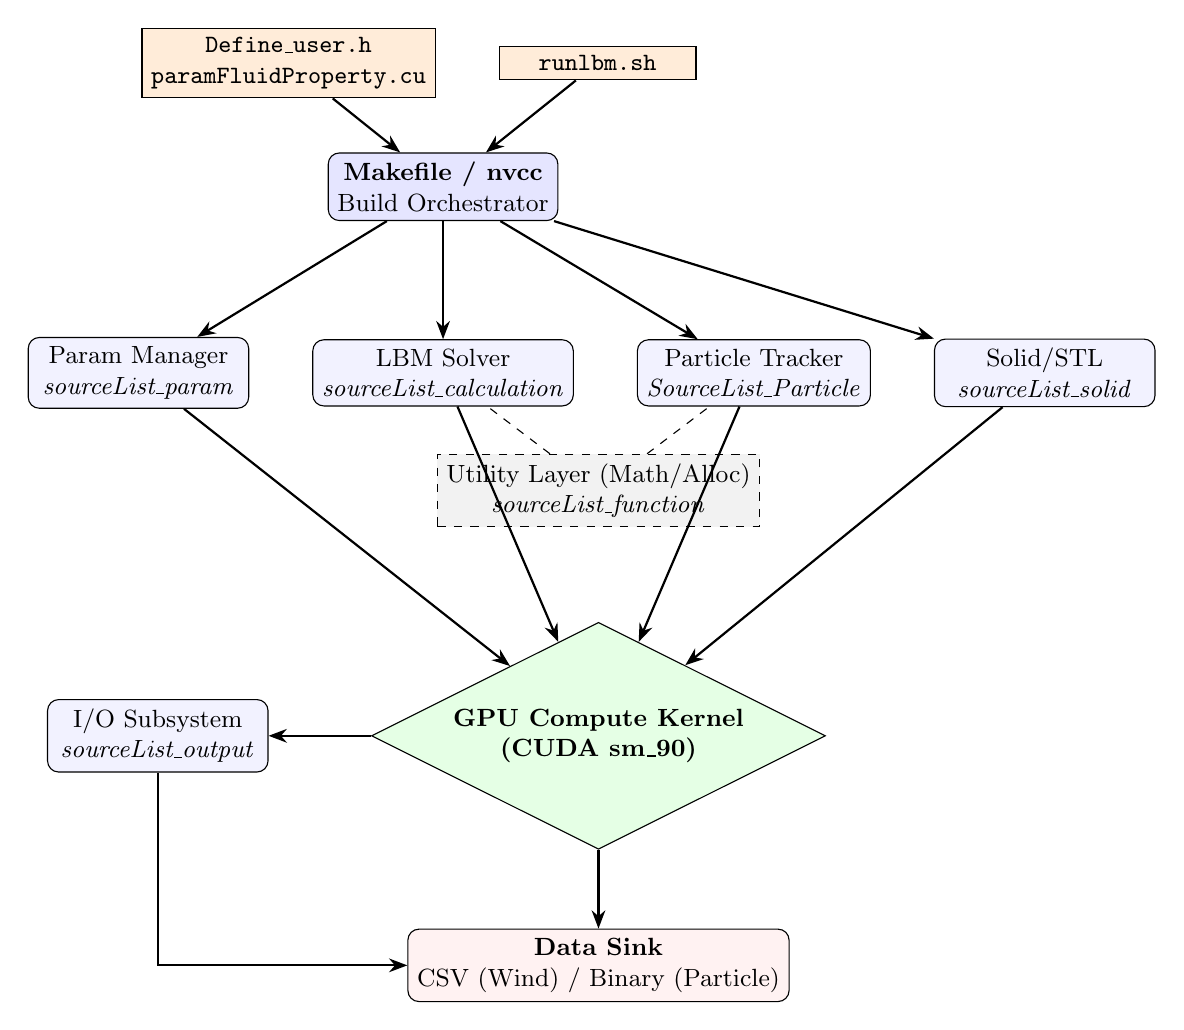
\begin{tikzpicture}[
        node distance=1.2cm and 0.8cm,
        box/.style={rectangle, draw, rounded corners, minimum width=2.8cm, minimum height=0.8cm, align=center, font=\small, fill=blue!5},
        header/.style={rectangle, draw, fill=orange!15, minimum width=2.5cm, font=\small\ttfamily, align=center},
        engine/.style={diamond, draw, fill=green!10, aspect=2, minimum width=3cm, font=\small\bfseries, align=center},
        util/.style={rectangle, draw, dashed, fill=gray!10, minimum width=2.5cm, font=\small, align=center},
        arrow/.style={-Stealth, thick}
    ]

        % 1. Input/Control Layer
        \node (config) [header] {Define\_user.h \\ paramFluidProperty.cu};
        \node (script) [header, right=of config] {runlbm.sh};
        \node (makefile) [box, below=0.8cm of $(config.south)!0.5!(script.south)$, fill=blue!10] {\textbf{Makefile / nvcc} \\ Build Orchestrator};

        % 2. Modular Source Layer (The .mak files)
        \node (lbm) [box, below=1.5cm of makefile] {LBM Solver \\ \textit{sourceList\_calculation}};
        \node (lpt) [box, right=of lbm] {Particle Tracker \\ \textit{SourceList\_Particle}};
        \node (param) [box, left=of lbm] {Param Manager \\ \textit{sourceList\_param}};
        \node (solid) [box, right=of lpt] {Solid/STL \\ \textit{sourceList\_solid}};
        
        % 3. Support Layer (The Function Library)
        \node (func) [util, below=0.6cm of $(lbm.south)!0.5!(lpt.south)$] {Utility Layer (Math/Alloc) \\ \textit{sourceList\_function}};

        % 4. Execution Core
        \node (gpu) [engine, below=1.2cm of func] {GPU Compute Kernel \\ (CUDA sm\_90)};

        % 5. Output Layer
        \node (output_mod) [box, left=of gpu, xshift=-0.5cm] {I/O Subsystem \\ \textit{sourceList\_output}};
        \node (data) [box, below=1cm of gpu, fill=red!5] {\textbf{Data Sink} \\ CSV (Wind) / Binary (Particle)};

        % Connections
        \draw [arrow] (config) -- (makefile);
        \draw [arrow] (script) -- (makefile);
        \draw [arrow] (makefile) -- (lbm);
        \draw [arrow] (makefile) -- (lpt);
        \draw [arrow] (makefile) -- (param);
        \draw [arrow] (makefile) -- (solid);
        
        % Functional layer interaction
        \draw [dashed] (func) -- (lbm);
        \draw [dashed] (func) -- (lpt);
        
        \draw [arrow] (lbm) -- (gpu);
        \draw [arrow] (lpt) -- (gpu);
        \draw [arrow] (param) -- (gpu);
        \draw [arrow] (solid) -- (gpu);
        
        \draw [arrow] (gpu) -- (output_mod);
        \draw [arrow] (output_mod) |- (data);
        \draw [arrow] (gpu) -- (data);
    \end{tikzpicture}
    \caption{System architecture of the LBM simulation framework}
    \label{fig:sys_arch}
\end{figure}

\begin{figure}[ht]
    \centering
    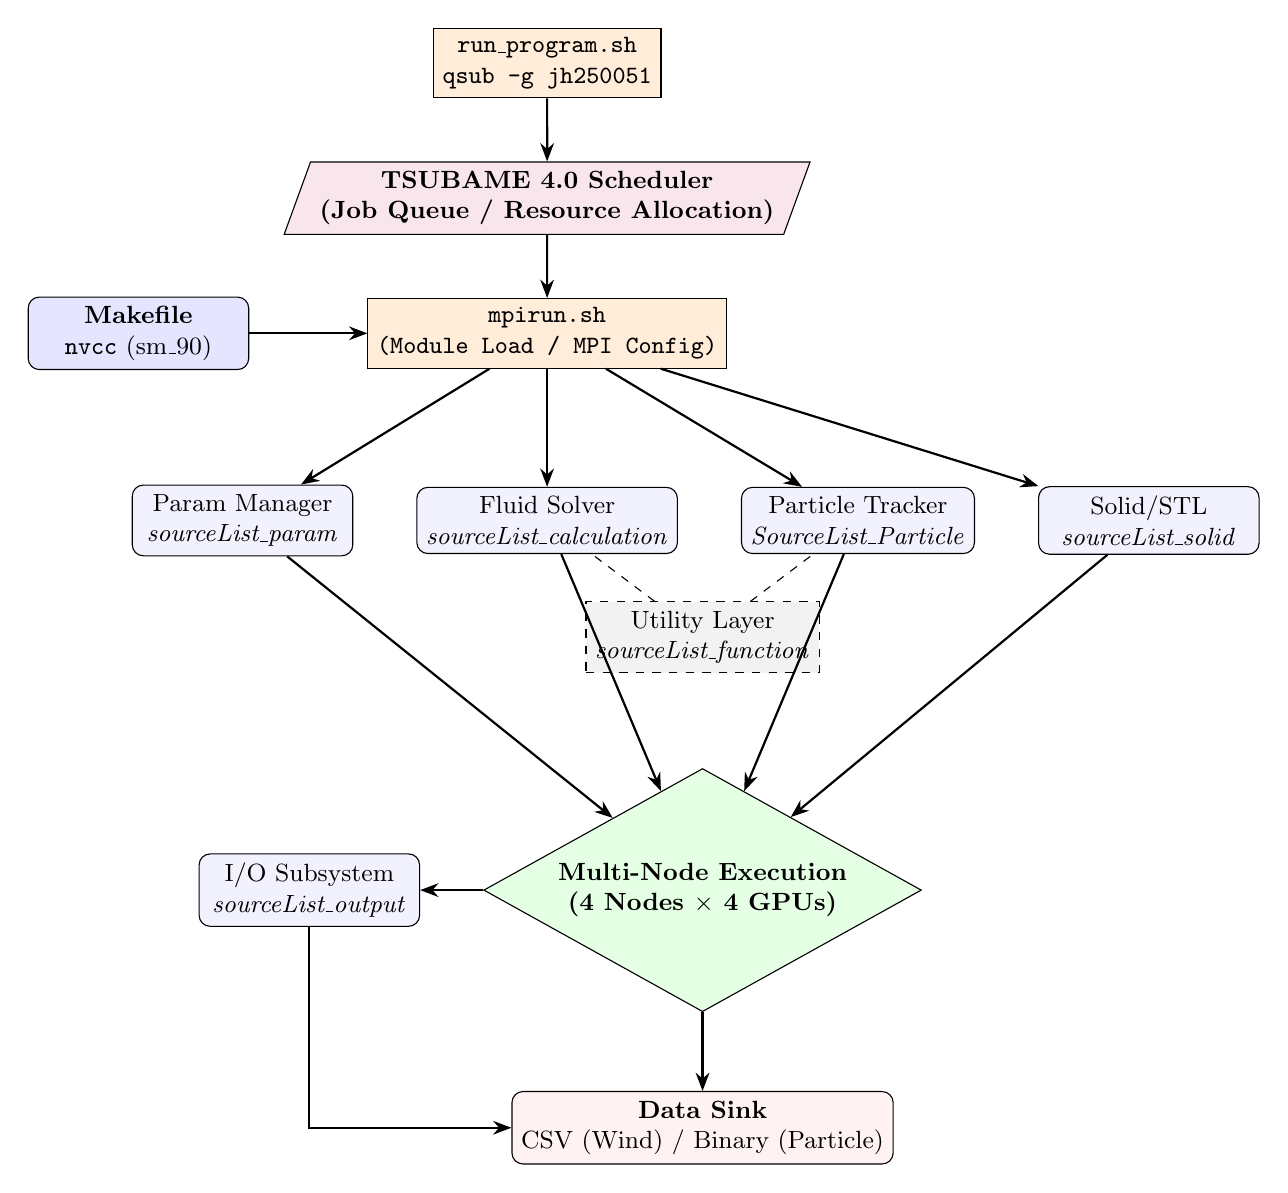
\begin{tikzpicture}[
        node distance=1cm and 0.8cm,
        box/.style={rectangle, draw, rounded corners, minimum width=2.8cm, minimum height=0.8cm, align=center, font=\small, fill=blue!5},
        header/.style={rectangle, draw, fill=orange!15, minimum width=2.5cm, font=\small\ttfamily, align=center},
        scheduler/.style={trapezium, trapezium left angle=70, trapezium right angle=110, draw, fill=purple!10, minimum width=3cm, font=\small\bfseries, align=center},
        engine/.style={diamond, draw, fill=green!10, aspect=1.8, minimum width=3.5cm, font=\small\bfseries, align=center},
        util/.style={rectangle, draw, dashed, fill=gray!10, minimum width=2.5cm, font=\small, align=center},
        arrow/.style={-Stealth, thick}
    ]

        % 1. Scheduler/Entry Layer
        \node (run_prog) [header] {run\_program.sh \\ \texttt{qsub -g jh250051}};
        \node (scheduler) [scheduler, below=0.8cm of run_prog] {TSUBAME 4.0 Scheduler \\ (Job Queue / Resource Allocation)};
        
        % 2. Batch Control Layer
        \node (mpirun_sh) [header, below=0.8cm of scheduler] {mpirun.sh \\ (Module Load / MPI Config)};
        \node (makefile) [box, left=1.5cm of mpirun_sh, fill=blue!10] {\textbf{Makefile} \\ \texttt{nvcc} (sm\_90)};

        % 3. Modular Source Layer
        \node (lbm) [box, below=1.5cm of mpirun_sh] {Fluid Solver \\ \textit{sourceList\_calculation}};
        \node (lpt) [box, right=of lbm] {Particle Tracker \\ \textit{SourceList\_Particle}};
        \node (param) [box, left=of lbm] {Param Manager \\ \textit{sourceList\_param}};
        \node (solid) [box, right=of lpt] {Solid/STL \\ \textit{sourceList\_solid}};
        
        % 4. Support Layer
        \node (func) [util, below=0.6cm of $(lbm.south)!0.5!(lpt.south)$] {Utility Layer \\ \textit{sourceList\_function}};

        % 5. High-Performance Execution
        \node (gpu) [engine, below=1.2cm of func] {Multi-Node Execution \\ (4 Nodes $\times$ 4 GPUs)};

        % 6. Output Layer
        \node (output_mod) [box, left=of gpu] {I/O Subsystem \\ \textit{sourceList\_output}};
        \node (data) [box, below=1cm of gpu, fill=red!5] {\textbf{Data Sink} \\ CSV (Wind) / Binary (Particle)};

        % Connections
        \draw [arrow] (run_prog) -- (scheduler);
        \draw [arrow] (scheduler) -- (mpirun_sh);
        \draw [arrow] (makefile) -- (mpirun_sh);
        
        \draw [arrow] (mpirun_sh) -- (lbm);
        \draw [arrow] (mpirun_sh) -- (lpt);
        \draw [arrow] (mpirun_sh) -- (param);
        \draw [arrow] (mpirun_sh) -- (solid);
        
        \draw [dashed] (func) -- (lbm);
        \draw [dashed] (func) -- (lpt);
        
        \draw [arrow] (lbm) -- (gpu);
        \draw [arrow] (lpt) -- (gpu);
        \draw [arrow] (param) -- (gpu);
        \draw [arrow] (solid) -- (gpu);
        
        \draw [arrow] (gpu) -- (output_mod);
        \draw [arrow] (output_mod) |- (data);
        \draw [arrow] (gpu) -- (data);

    \end{tikzpicture}
    \caption{System architecture of the LBM simulation framework executed using the TSUBAME 4.0 Supercomputer}
    \label{fig:tsubame_arch}
\end{figure}

\subsection{Simulation Parameters and Case Setup}
The specific configurations for the validation and research cases are summarized in Table~\ref{tab:simulation_cases_full}. These cases represent the transition from local prototyping to large-scale supercomputer execution.

\begin{table}[ht]
\centering
\caption{Detailed Simulation Case Parameters}
\label{tab:simulation_cases_full}
\resizebox{\textwidth}{!}{%
\begin{tabular}{lcccccccc}
\hline
\textbf{Case} & \textbf{Environment} & \textbf{Domain Size ($x, y, z$ in m)} & \textbf{Duration (s)} & \textbf{Approach} & \textbf{$H_{cube}$ (m)} & \textbf{$z_0$ (m)} & \textbf{$U_0$ (m/s)} & \textbf{Flow Rate} \\ \hline
1 & Local Server & $832 \times 384 \times 240$ & 2400 & No & -- & 0.001 & 6.0 & 150 p/s \\
2 & TSUBAME 4.0 & $4352 \times 384 \times 320$ & 6000 & Yes & 8 & 0.001 & 6.0 & 150 p/s \\
3 & TSUBAME 4.0 & $4352 \times 384 \times 320$ & 6000 & Yes & 16 & 0.001 & 6.0 & 150 p/s \\
4 & TSUBAME 4.0 & $4352 \times 384 \times 320$ & 6000 & Yes & 20 & 0.001 & 6.0 & 150 p/s \\
5 & TSUBAME 4.0 & $4352 \times 384 \times 320$ & 6000 & Yes & 24 & 0.001 & 6.0 & 150 p/s \\
6 & TSUBAME 4.0 & $4352 \times 384 \times 320$ & 6000 & Yes & 32 & 0.001 & 6.0 & 150 p/s \\
7 & TSUBAME 4.0 & $4352 \times 384 \times 320$ & 6000 & Yes & 16 & 0.1 & 6.0 & 150 p/s \\
8 & TSUBAME 4.0 & $4352 \times 384 \times 320$ & 6000 & Yes & 20 & 0.1 & 6.0 & 150 p/s \\ \hline
\end{tabular}%
}
\end{table}

\subsection{Physical and Dimensionless Parameters}
To ensure the dynamic similarity between the wind tunnel experiment and the Lattice Boltzmann Method (LBM) simulation, the Reynolds number ($Re$) is calculated. This dimensionless value represents the ratio of inertial forces to viscous forces.\textbf{Reynolds Number ($Re$)}For this study, the characteristic length is defined as the building height $H$, and the velocity is the wind speed at that height $U_H$.

\begin{equation}
    Re = \frac{U_H \cdot H}{\nu}
\end{equation}

While the experimental $Re_{exp}$ is $4.3 \times 10^4$, the LBM simulation on TSUBAME 4.0 operates at a significantly higher effective Reynolds number ($Re_{LBM} \approx 2.09 \times 10^7$), reflecting the high-fidelity nature of the Large Eddy Simulation (LES) approach.

\subsubsection{Wind and Turbulence Data Post-Processing and Statistical Analysis}

The Large Eddy Simulation (LES) results were post-processed to extract time-averaged wind statistics and turbulence characteristics. The simulation domain was decomposed into four parallel sub-domains (indexed 0000 to 0003) for computational efficiency on the TSUBAME 4.0 supercomputer. 

Data analysis focused primarily on the fourth sub-domain (0003), which contains the building model and the validation points of interest, excluding the approach flow sections (0000–0002).

\textbf{Data Structure and Extraction}
Wind field data were exported as planar cross-sections ($xy$-planes) at various vertical grid heights ($k$). The raw output files follow a stacked structure where each height level is preceded by a header indicating the vertical grid index, followed by a $192 \times 544$ matrix representing the spanwise ($y$) and streamwise ($x$) velocity components. On the small domain simulation (Case 1), the data structure is similar, except for the inexistence of the approach section. Thus, for the small domain simulation, only one sub-domain, 0000, exists, and the analysis is done over that sub-domain only.

The analysis utilizes time-averaged velocity components ($\bar{u}, \bar{v}, \bar{w}$) and second-order velocity moments ($\overline{u^2}, \overline{v^2}, \overline{w^2}$), averaged over 540,000 time steps (equivalent to 5,400 physical seconds) to ensure statistical convergence. These variables correspond to the output files \texttt{xy\_um}, \texttt{xy\_vm}, \texttt{xy\_wm} (first-order moments) and \texttt{xy\_uu}, \texttt{xy\_vv}, \texttt{xy\_ww} (second-order moments).

\textbf{Turbulence Statistics}
To evaluate the turbulent flow characteristics, Reynolds stresses were calculated by subtracting the square of the mean velocity from the mean of the squared velocity. The streamwise ($\langle u'^2 \rangle$), spanwise ($\langle v'^2 \rangle$), and vertical ($\langle w'^2 \rangle$) Reynolds normal stresses were derived as follows:

\begin{align}
    \langle u'^2 \rangle &= \overline{u^2} - (\bar{u})^2 \\
    \langle v'^2 \rangle &= \overline{v^2} - (\bar{v})^2 \\
    \langle w'^2 \rangle &= \overline{w^2} - (\bar{w})^2 
\end{align}

\textbf{Root Mean Square (RMS) Fluctuations}
The Root Mean Square (RMS) velocity fluctuations, which indicate the intensity of turbulence in each direction, were calculated and normalized by the reference approach flow velocity ($U_H$) at building height $H$:

\begin{equation}
    u_{rms} = \frac{\sqrt{\langle u'^2 \rangle}}{U_H}, \quad v_{rms} = \frac{\sqrt{\langle v'^2 \rangle}}{U_H}, \quad w_{rms} = \frac{\sqrt{\langle w'^2 \rangle}}{U_H}
\end{equation}

\textbf{Turbulence Kinetic Energy (TKE)}
The Turbulence Kinetic Energy ($k$), representing the mean kinetic energy per unit mass associated with eddies in the turbulent flow, was computed as half the sum of the Reynolds normal stresses:

\begin{equation}
    k = \frac{1}{2} \left( \langle u'^2 \rangle + \langle v'^2 \rangle + \langle w'^2 \rangle \right)
\end{equation}

To handle numerical stability during post-processing, a constraint was applied such that any negative stress values resulting from floating-point errors were clamped to zero before the square root operation ($\text{max}(0, \sigma^2)$). All statistical results were mapped to the physical domain coordinates to facilitate direct comparison with the Architectural Institute of Japan (AIJ) wind tunnel experimental benchmarks.

\subsubsection{Lagrangian Particle Data Post-Processing and Statistical Analysis}

Due to the high temporal and spatial resolution of the Lagrangian tracking, the raw output is generated in a compact binary format to minimize I/O overhead. To translate these large-scale datasets into physically interpretable results, a dedicated post-processing suite was developed in C++. This suite follows a modular architecture, where specific physical quantities are computed by discrete analytical engines coordinated through a central execution framework. The post-processing workflow is orchestrated by a multi-threaded C++ executable, compiled via a modular \texttt{Makefile} that links specialized modules for density calculation, flux analysis, vertical profiling, and flux footprint prediction (FFP). The system is designed for high flexibility; rather than hard-coding simulation parameters, the tool utilizes a Command-Line Interface (CLI) where domain dimensions, grid size, time steps, and output intervals are passed as dynamic arguments at runtime. This allows the same analytical core to be applied across various experimental cases, ranging from local isolated building tests to large-scale urban simulations without the need for frequent re-compilation. Execution is managed through batch scripts (\texttt{run.bat}) For instance, the framework can simultaneously extract particle density profiles at specified heights ($z_{out}$) and compute the source area contributions at defined sensor locations. By leveraging OpenMP for multi-threading (\texttt{OMP\_NUM\_THREADS}), the post-processor efficiently iterates through millions of Lagrangian trajectories stored in the binary files, aggregating them into averaged statistical summaries (CSV or text format) suitable for final visualization in Python.

\subsection{Turbulence and Dispersion Modeling}

\textbf{Normalized Concentration ($C_{norm}$)} To allow for a direct comparison between experimental gas data and the Lagrangian particle model, concentration values are normalized based on the flow rate $Q$, velocity $U_H$, and building scale $H$.

\begin{equation}
    C_{norm} = \frac{C_o \cdot U_H \cdot H^2}{Q}
\end{equation}

\subsection{Statistical Validation Metrics}
Following the AIJ guidelines for urban wind environments, four metrics are used to compare the predicted values ($P_i$) against the observed experimental data ($O_i$).\textbf{Hit Rate ($q$)}The Hit Rate measures the reliability of the model. A data point is a "hit" if the prediction is within a relative tolerance $D$ (usually 0.25) or an absolute tolerance $W$ (usually 0.05).

\begin{equation}q = \frac{1}{N} \sum_{i=1}^{N} n_i, \quad n_i = 
    \begin{cases} 
        1 & \text{if } \left| \frac{P_i - O_i}{O_i} \right| \le D \text{ or } |P_i - O_i| \le W \\ 0 & \text{else} 
    \end{cases}
\end{equation}

\textbf{Factor of Two (FAC2)} FAC2 is a robust measure of the overall spread. It checks if the predicted value is between half and double the observed value.

\begin{equation}\text{FAC2} = \frac{1}{N} \sum_{i=1}^{N} n_i, \quad n_i = 
    \begin{cases} 
        1 & \text{if } 0.5 \le \frac{P_i}{O_i} \le 2.0 \\ 0 & \text{else} 
    \end{cases}
\end{equation}

\textbf{Error Metrics (MAE and RMSE)} The Mean Absolute Error (MAE) provides the average magnitude of the errors, while the Root Mean Square Error (RMSE) gives a higher weight to large outliers, providing a stricter assessment of simulation accuracy.

\begin{equation}
    \text{MAE} = \frac{1}{N} \sum_{i=1}^{N} |P_i - O_i|, \quad \text{RMSE} = \sqrt{\frac{1}{N} \sum_{i=1}^{N} (P_i - O_i)^2}\end{equation}

\newpage
\include{sections/results_discussion}
\include{sections/conclusion}

\printbibliography{}
\end{document}